\section{Ongoing Studies and Plans}
\label{sec:ongoing}

In this section, we discuss the ongoing studies on the deficit in
the reconstructed energy, and the proposed treatments which is being
tested.
In addition, we outline the plans on the shower reconstruction in
near future, which aim to cope with events with more complicated
topologies.

% -----------------------------------------------------------------------
\subsection{Energy Deficit}
\label{sec:energy_deficit}

As mentioned in~\Cref{sec:data_pi0}, the energy deficit in the reconstructed
showers has the greatest impact in the reconstructed $\pizero$ mass.
First of all, we try to disentangle the impact of clustering inefficiency
and that of other possible sources.
Starting with the single electron sample,
we merge all reconstructed hits in an event into a PFParticle
and reconstruct the energy of the PFParticle with the same algorithm
mentioned in~\Cref{sec:shr_calorimetry}.
Such a PFParticle represents the perfect clustering, as all the hits
in a single particle event come from an original particle.\\
\\
\Cref{fig:energy_deficiency} displays the energy resolution (defined 
in~\Cref{sec:shr_quality})
in the three wire planes with the four combinations of the wire configuratios 
and the hit producers,
\begin{itemize}
\item Wire configuration
  \begin{itemize}
  \item all good wires (G): all the wires are good wires,
  \item bad wires (B): using the bad wire configuration according to
        the database,
  \end{itemize}
\item Hit producer
  \begin{itemize}
  \item gaushit (Gaushit): hits produced by the Gaussian hit finder;
        i.e. all the hits in an event,
  \item pandoraCosmicsKHitRemoval (PandoraCRm): hits produced by
        pandoraCosmics, which removes the hits from cosmic rays~\cite{DocDB5828}.
  \end{itemize}
\end{itemize}
The peak of energy resolution in all the combinations is offset
from zero by about 15\%, indicating the amount of the energy deficit
beyond clustering inefficiency.
This might attribute to energy calibration, and/or small amount of 
charge deposition which does not pass the threshold in the hit finder.
Furthermore, the existence of bad wires degrades the resolution, but
does not have a significant impact on the energy deficiency.

% --------------------------------------------------------------------
% Figure: Energy checks
\begin{figure}[htbp]
\begin{center}
\includegraphics[width=0.45\textwidth]{figs/ongoing/energy/EnergyResU.eps}
\includegraphics[width=0.45\textwidth]{figs/ongoing/energy/EnergyResV.eps}
\includegraphics[width=0.45\textwidth]{figs/ongoing/energy/EnergyResY.eps}
\caption{The energy resolution of all reconstructed hits compared to the
true deposited energy in the U, V, and Y wire planes.
The legends are explained in the text.}
\label{fig:energy_deficiency}
\end{center}
\end{figure}
% --------------------------------------------------------------------


% -----------------------------------------------------------------------
\subsection{Clustering Inefficiency}
\label{sec:clustering_ineff}

\Cref{fig:clustering_deficiency} suggests (5-10)\% of energy deficit 
causing by clustering
inefficiency in addition to the 15\% described in~\Cref{sec:energy_deficit}.
It is noticable Pandora creates multiple small PFParticles in 
a single electron/photon event, and leaves a number of hits unclustered.
To retrieve the energy, we start with merging PFParticles, and then
perform a reclustering algorithm to collect the unclustered hits.
\Cref{sec:merging,sec:adding_hits} sketch the two steps respectively.

% --------------------------------------------------------------------
% Figure: Clustering
\begin{figure}[htbp]
\begin{center}
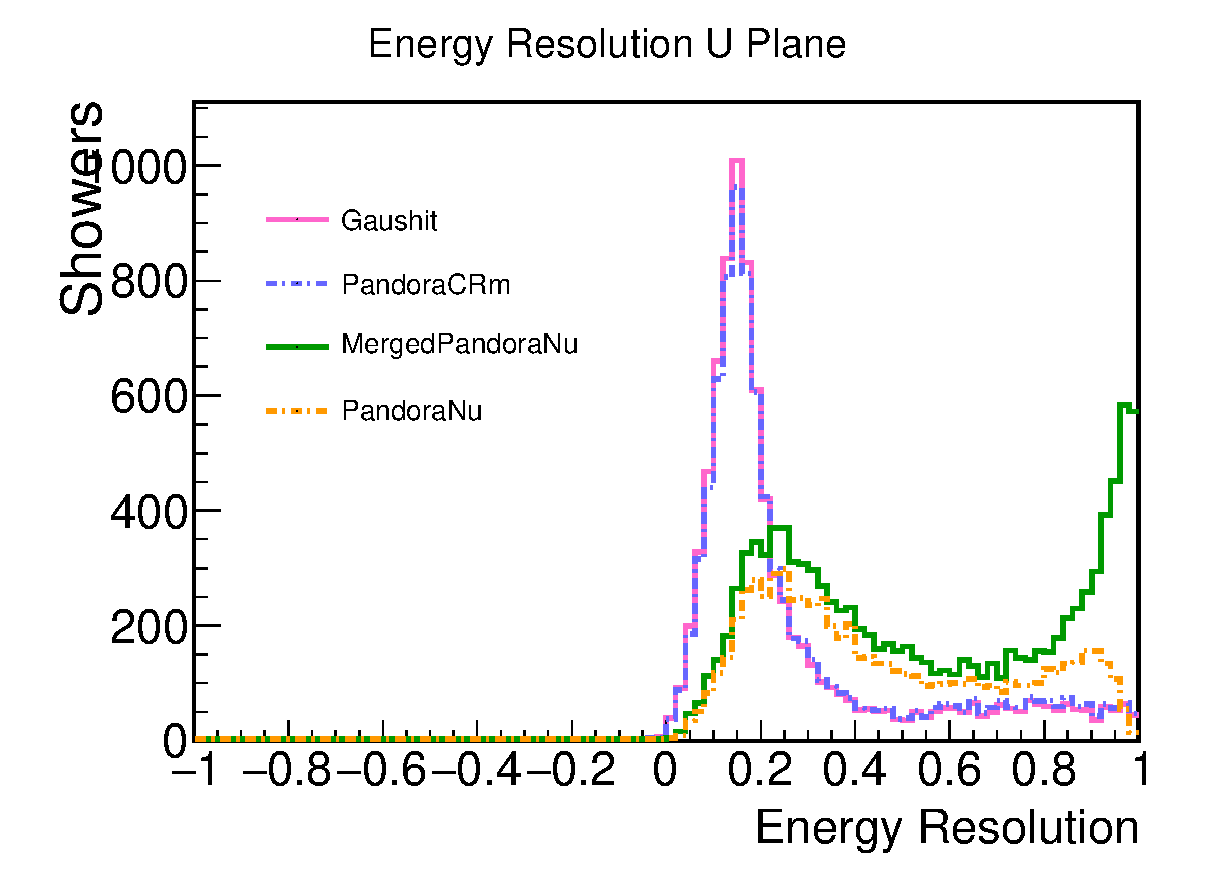
\includegraphics[width=0.45\textwidth]{figs/ongoing/clustering/EnergyResU.eps}
\includegraphics[width=0.45\textwidth]{figs/ongoing/clustering/EnergyResV.eps}
\includegraphics[width=0.45\textwidth]{figs/ongoing/clustering/EnergyResY.eps}
\caption{The energy resolution of all reconstructed hits, clustered hits 
compared to the
true deposited energy in the U, V, and Y wire planes.
The legends are explained in the text.}
\label{fig:clustering_deficiency}
\end{center}
\end{figure}
% --------------------------------------------------------------------

% -----------------------------------------------------------------------
\subsubsection{Merging PFParticles}
\label{sec:merging}

Not only does Pandora create multiple small PFParticles in
the single electron, photon samples,
but it also identifies a number of PFParticles as tracks.
Aiming to investigate how much energy would be retrieved by merging
multiple PFParticles, we include both shower-like and track-like
PFParticles in this study.\\
\\
The current merging algorithm is designed to cope with the showers
following the photons produced by Bremsstrahlung,
which is often observed in event displays,
and can potentially reduce the impact of bad wires.
PFParticles are merged if either of the following requirements is met:
\begin{itemize}
\item the vertex of the less energetic PFParticle falls within the 
      cone of the other
\item the principal component axis of one PFParticle is aligned
      within the cone of the other
\end{itemize}
The cone size in this study is set to the opening angle of the shower,
but is subject to be optimized in the future.\\
\\
The shower reconstruction based on merged PFParticles are compared
to that on shower-like ones in~\Cref{fig:shr_quality_merged_single_e,fig:shr_quality_merged_single_gamma,fig:mpi0_merged_single_pi0},
for the single electron, photon, and $\pizero$ samples, respectively.
Using merged PFParticles significantly improve the efficiency on
shower reconstruction and thereby the $\pizero$ mass reconstruction,
as there are nonnegligible PFParticles in these samples identified
as tracks.
Nonetheless, the energy deficiency persists with a similar amount in
the reconstruction based on merged PFParticles, suggesting the broken
PFParticles are not the main source of clustering inefficiency.\\
\\
% --------------------------------------------------------------------
% Figure: Shower quality for single e events
\begin{figure}[htbp]
\begin{center}
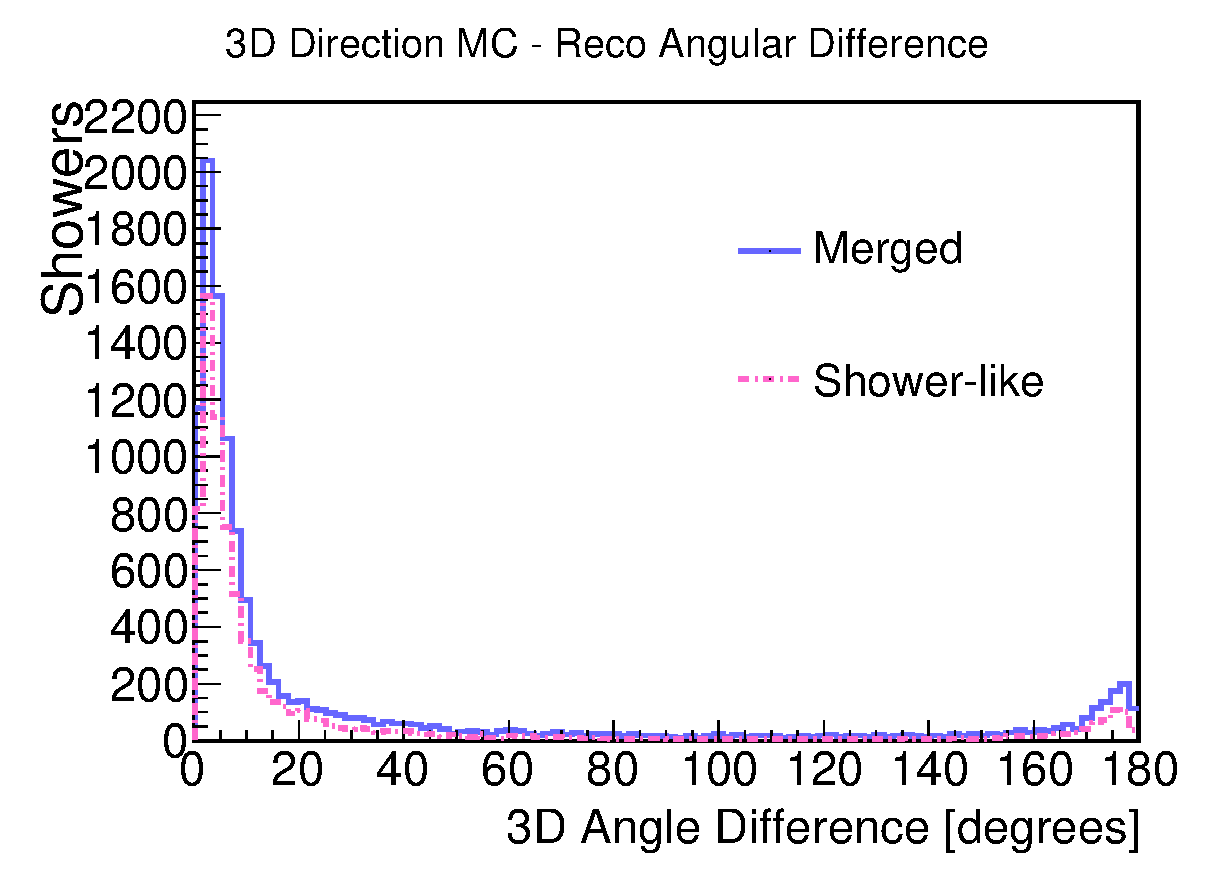
\includegraphics[width=0.3\textwidth]{figs/ongoing/eminus/AngleDiff.eps}
\includegraphics[width=0.3\textwidth]{figs/ongoing/eminus/StartingPointAcc.eps}
\includegraphics[width=0.3\textwidth]{figs/ongoing/eminus/Length.eps}
\includegraphics[width=0.3\textwidth]{figs/ongoing/eminus/ClusterEffU.eps}
\includegraphics[width=0.3\textwidth]{figs/ongoing/eminus/ClusterEffV.eps}
\includegraphics[width=0.3\textwidth]{figs/ongoing/eminus/ClusterEffY.eps}
\includegraphics[width=0.3\textwidth]{figs/ongoing/eminus/EnergyResU.eps}
\includegraphics[width=0.3\textwidth]{figs/ongoing/eminus/EnergyResV.eps}
\includegraphics[width=0.3\textwidth]{figs/ongoing/eminus/EnergyResY.eps}
\includegraphics[width=0.3\textwidth]{figs/ongoing/eminus/dEdxU.eps}
\includegraphics[width=0.3\textwidth]{figs/ongoing/eminus/dEdxV.eps}
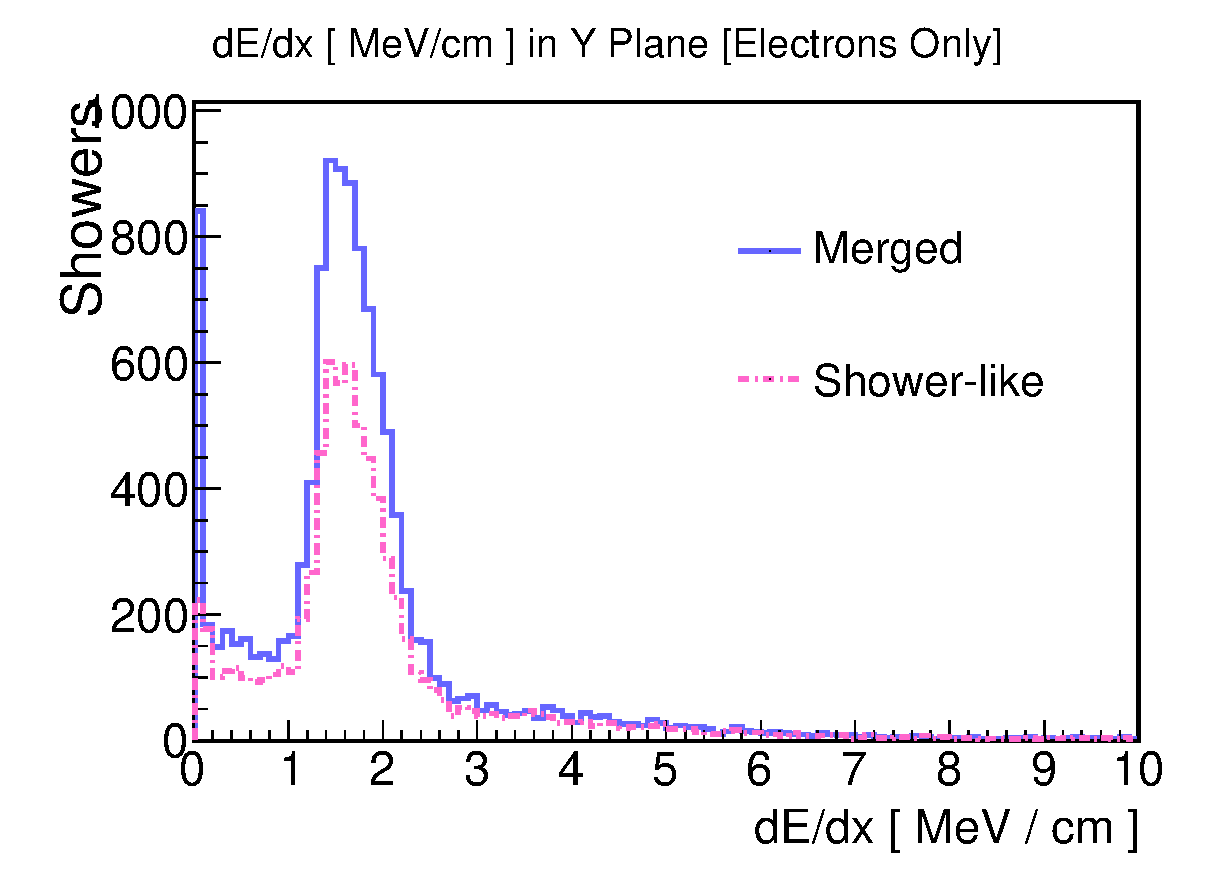
\includegraphics[width=0.3\textwidth]{figs/ongoing/eminus/dEdxY.eps}
\includegraphics[width=0.3\textwidth]{figs/ongoing/eminus/dQdxU.eps}
\includegraphics[width=0.3\textwidth]{figs/ongoing/eminus/dQdxV.eps}
\includegraphics[width=0.3\textwidth]{figs/ongoing/eminus/dQdxY.eps}
\includegraphics[width=0.3\textwidth]{figs/ongoing/eminus/NRecoShowers.eps}
\caption{Shower quality reconstructed from merged and shower-like PFParticles
in the single electron MC samples.}
\label{fig:shr_quality_merged_single_e}
\end{center}
\end{figure}
% -------------------------------------------------------------------
% --------------------------------------------------------------------
% Figure: Shower quality for single gamma events
\begin{figure}[htbp]
\begin{center}
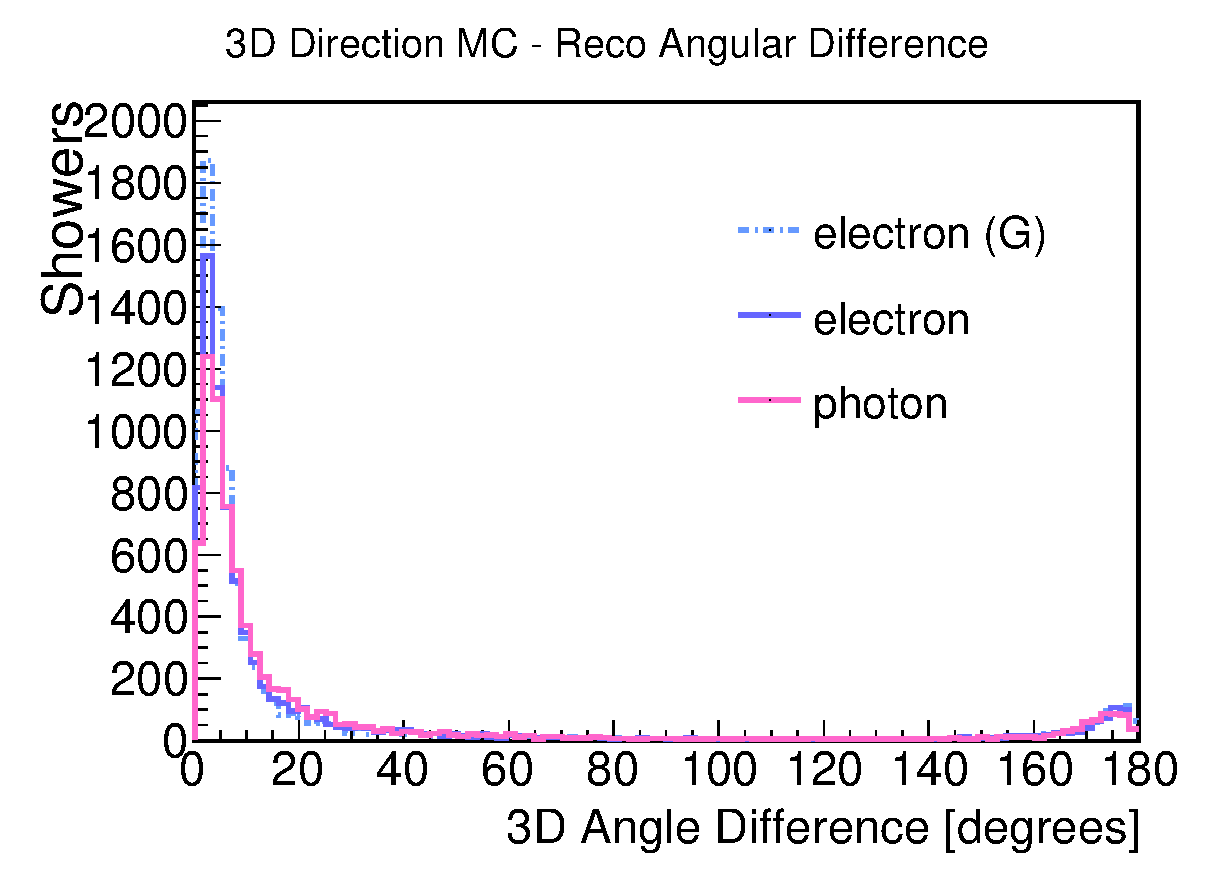
\includegraphics[width=0.3\textwidth]{figs/ongoing/gamma/AngleDiff.eps}
\includegraphics[width=0.3\textwidth]{figs/ongoing/gamma/StartingPointAcc.eps}
\includegraphics[width=0.3\textwidth]{figs/ongoing/gamma/Length.eps}
\includegraphics[width=0.3\textwidth]{figs/ongoing/gamma/ClusterEffU.eps}
\includegraphics[width=0.3\textwidth]{figs/ongoing/gamma/ClusterEffV.eps}
\includegraphics[width=0.3\textwidth]{figs/ongoing/gamma/ClusterEffY.eps}
\includegraphics[width=0.3\textwidth]{figs/ongoing/gamma/EnergyResU.eps}
\includegraphics[width=0.3\textwidth]{figs/ongoing/gamma/EnergyResV.eps}
\includegraphics[width=0.3\textwidth]{figs/ongoing/gamma/EnergyResY.eps}
\includegraphics[width=0.3\textwidth]{figs/ongoing/gamma/dEdxU.eps}
\includegraphics[width=0.3\textwidth]{figs/ongoing/gamma/dEdxV.eps}
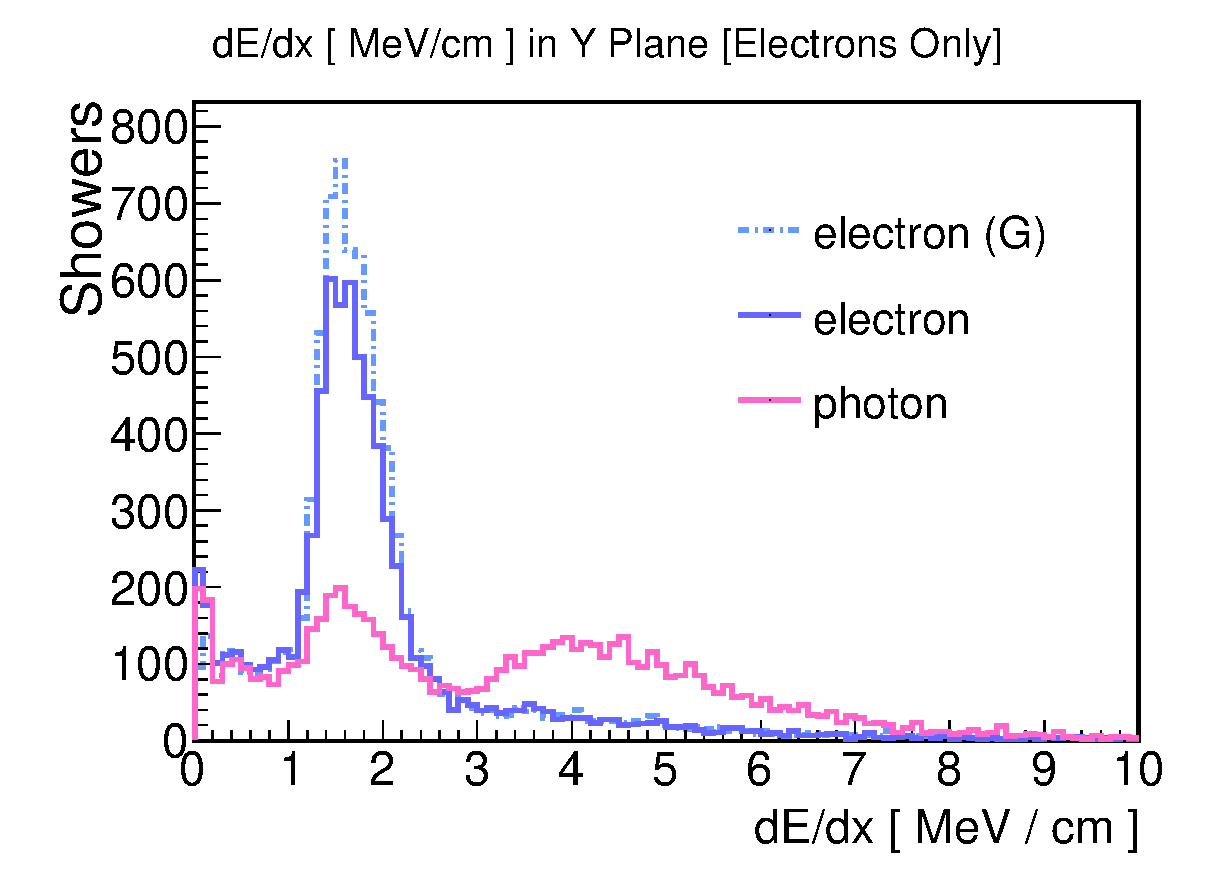
\includegraphics[width=0.3\textwidth]{figs/ongoing/gamma/dEdxY.eps}
\includegraphics[width=0.3\textwidth]{figs/ongoing/gamma/dQdxU.eps}
\includegraphics[width=0.3\textwidth]{figs/ongoing/gamma/dQdxV.eps}
\includegraphics[width=0.3\textwidth]{figs/ongoing/gamma/dQdxY.eps}
\includegraphics[width=0.3\textwidth]{figs/ongoing/gamma/NRecoShowers.eps}
\caption{Shower quality reconstructed from merged and shower-like PFParticles
in the single photon MC samples.}
\label{fig:shr_quality_merged_single_gamma}
\end{center}
\end{figure}
% --------------------------------------------------------------------
% --------------------------------------------------------------------
% Figure: pi0 mass
\begin{figure}[htbp]
\begin{center}
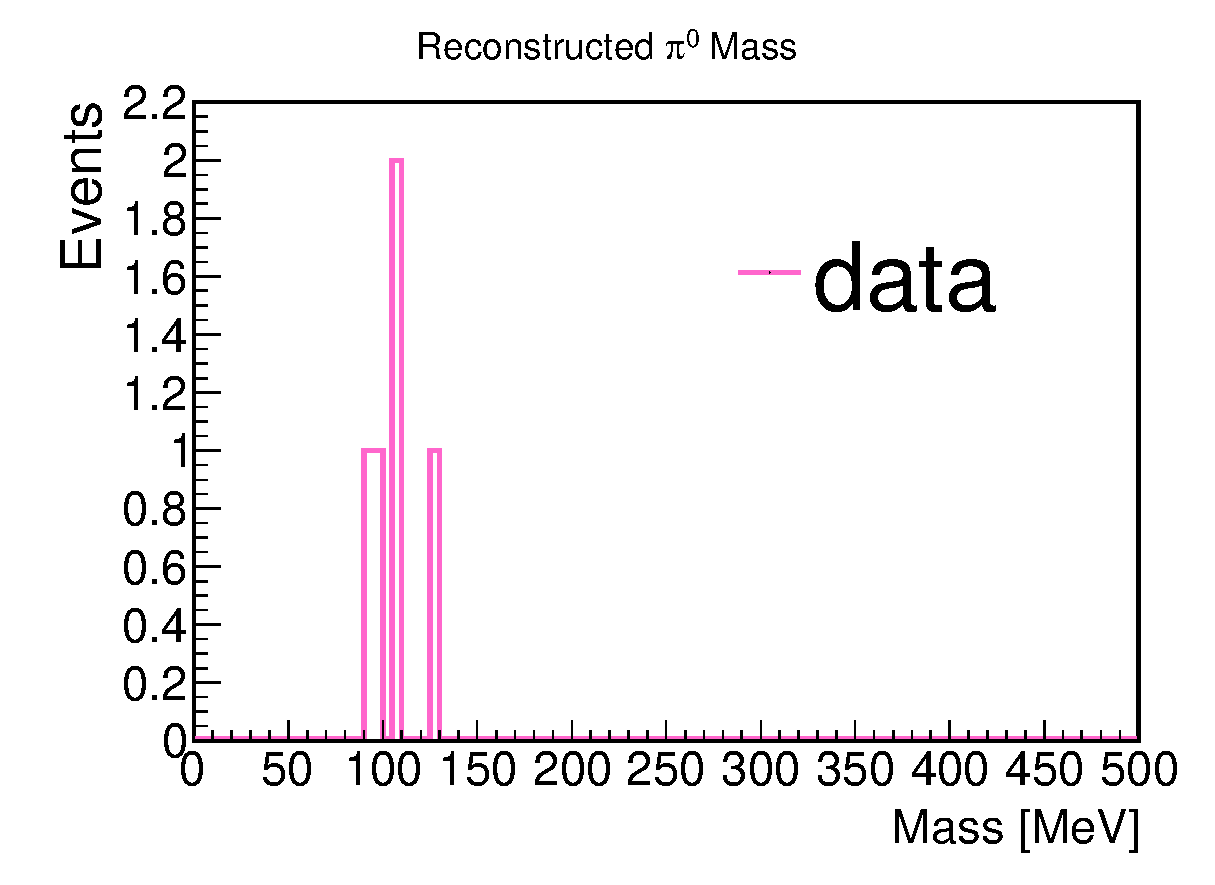
\includegraphics[width=0.75\textwidth]{figs/ongoing/pi0/RecoPi0Mass.eps}
\caption{Reconstructed $\pizero$ mass distribution from merged and
shower-like PFParticles in the single $\pizero$ MC sample.}
\label{fig:mpi0_merged_single_pi0}
\end{center}
\end{figure}
% --------------------------------------------------------------------
Incidentally,
the energy resolution distributions for merged PFParticles have a 
low energy tail (a small peak near one) owing to the fact that
small PFParticles are often identified as tracks, and are taken into
account in this case.

% -----------------------------------------------------------------------
\subsubsection{Adding Unclustered Hits}
\label{sec:adding_hits}

To further investigate the key source of clustering inefficiency
and retrieve unreconstructed energy,
we add unclustered hits into the hit collection associated to a 
PFParticle according to a cone algorithm.
This study is currently underway.

% -----------------------------------------------------------------------
\subsection{Short Term Plans}
\label{sec:plans}

We plan to complete the studies on the BNB neutrino and cosmogenic
background simulation as mentioned in~\Cref{sec:bnb},
as well as to perform low level checks (e.g.~\cite{DocDB5814}) 
on energy calibration
and other possible sources of energy deficiency.
Moreover, a few aspects to potentially solidify the shower reconstruction
are sketched below.
\begin{itemize}
\item {\bf PFParticle Merging and Reclustering} \\
We will optimize the parameters for PFParticle merging algorithms,
and start testing as well as further developing the reclustering algorithms
which add unclustered hits into PFParticles and would possibly
eliminate the energy deficiency.
The algorithms would possibly be integrated into the Pandora
toolkit in as a mid-term goal.

\item {\bf Shower Profiling} \\
It is likely that merging and reclustering algorithms would not
retrieve all the energy deposition of a shower.
We thereby plan to study the profile of showers and develop
correction factors accordingly.

\item {\bf Track-Shower Identification} \\
From the studies in~\Cref{sec:merging}, we notice
a nonnegligible fraction of PFParticles originating from an 
electromagnetic particle is identified as a track by Pandora.
The track-shower identification thereby needs to be modified.
We will examine the features of tracks and showers based on
simulation and develop a track/shower determination.

\item {\bf Electron-Photon Separation} \\
As shown in~Fig.x, the electron-photon separation in
dE/dx needs to be improved such that efficiently distinguishing 
those two particles can be achieved.
By further investigating the features of showers we may be able 
to optimize or develop algorithms for dE/dx.

\item {\bf $\pizero$ Mass Reconstruction} \\
In this study we reconstruct the $\pizero$ mass by
simply utilizing the hierarchy feature of the 
Pandora outputs.
We will try the algorithm stated in~\cite{DocDB5520}, examine
the efficiency in both the approaches, and possibly develop
other algorithms.
\end{itemize}

